%%%%%%%%%%% Aquí va la solución al problema 4.
\newpage
\textbf{\textcolor{MidnightBlue}{4.}} Da una ejecución del algoritmo 3 para $n=4$ procesos y
$t=1$ fallas bizantinas, en la que los procesos correctos no llegue a un consenso, a pesar de
que los cuatro procesos, íncluido el Bizantino, empiecen con la misma propuesta y el bizantino
sea el último de los coordinadores de la ejecución. Explica tu respuesta.

\begin{center}
    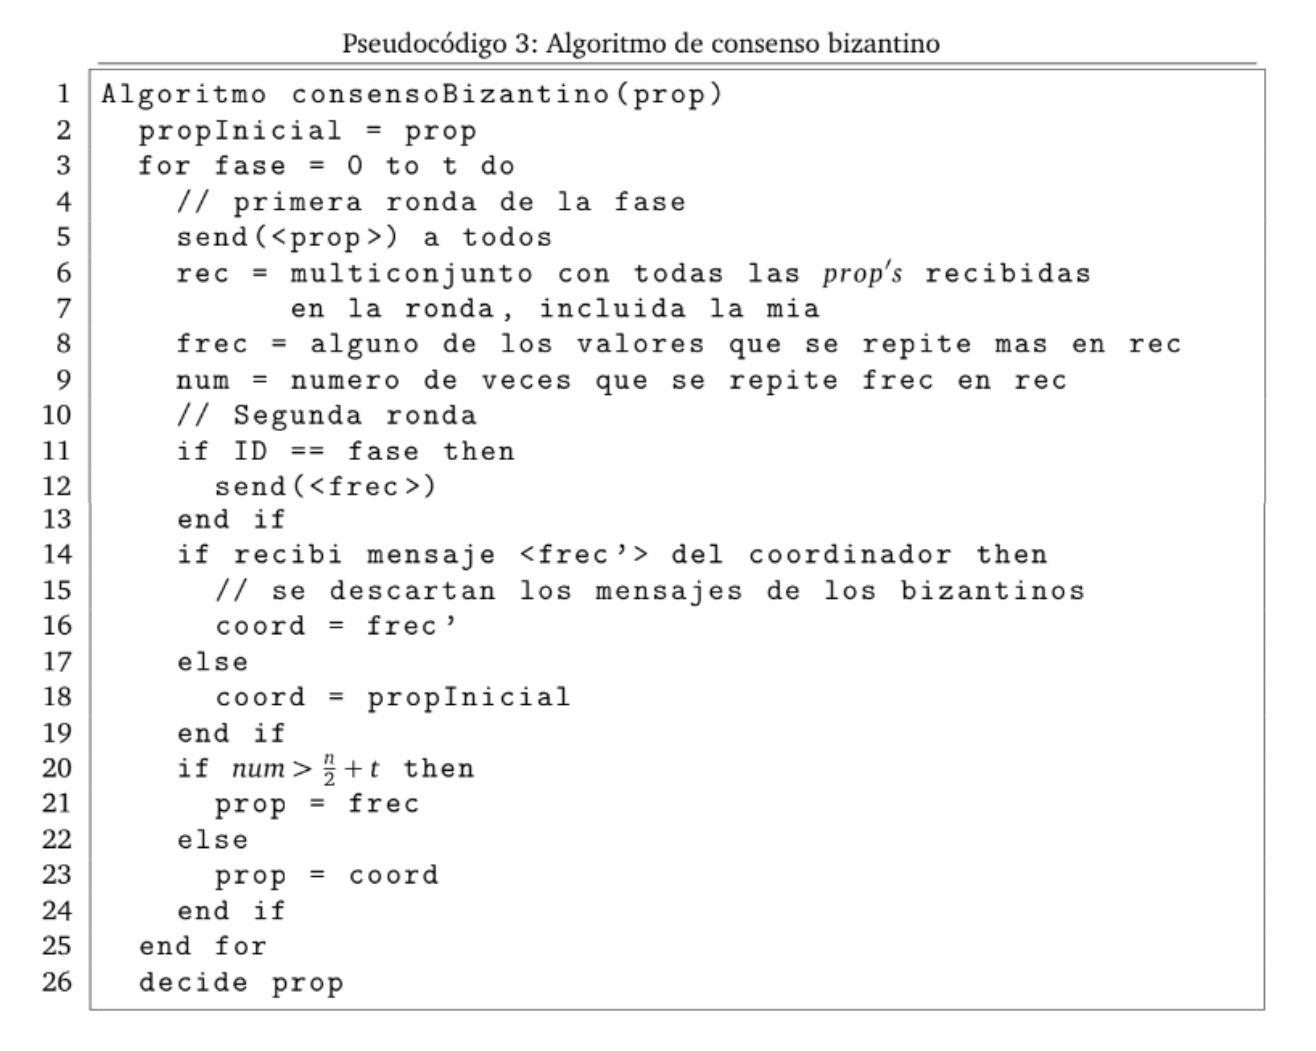
\includegraphics[scale=0.35]{consensoBizantino.png}
    \end{center}

Sabemos que el algoritmo soluciona el problema para $t<\frac{n}{4}$, donde $n$ son los proceso del
sistema, como sabemos que se ejecuta por fases de $2$ rondas, dado que se quiere hacer la ejecución
con $n=4$ y con $t=1$ fallos bizantinos, no es posible hacer que estos no lleguen a un consenso.
Dado que siempre estos procesos correctos:
\begin{itemize}
    \item Siempre decidirán un valor.
    \item De tener una propuesta inicial $v$, entonces sólo decidirán $v$.
    \item Siempre las decisiones de estos, son iguales.
\end{itemize}

Pero, podemos asegurar que de tener un proceso de más, donde sea con $n=5$ procesos y $t=1$ fallas
bizantinas es posible que no lleguen a un consenso. De misma forma podría ser que de tener $n=4$
procesos y $t=2$ fallas bizantinas es posible que no lleguen a un consenso. Esto debido a que no
existe un algoritmo, si $t\geq \frac{n}{3}$\\

Se anexa ejemplo de ejecución con $n=4$ y una falla bizantina. (Siempre se llega a un consenso).
\begin{center}
    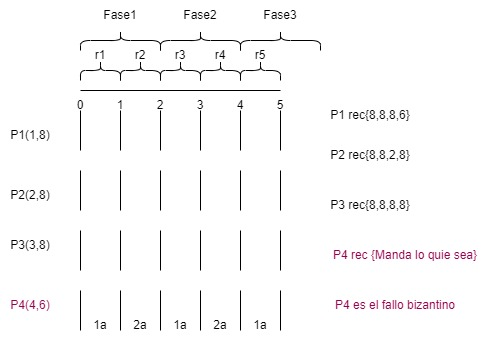
\includegraphics[scale=0.6]{Grapho.jpeg}
    \end{center}
